\chapter{Kempe chains and Routing graphs}
The following proofs are reformulations of those presented in \cite{matthias_2022}.

\begin{thm}
    K has property (*) if and only if every component of K has it.
\end{thm}

\begin{proof} 
\label{thm:first}
    \textbf{(\(\Rightarrow\))} If \(K\) has property (*) then all components of $K$ have property (*)
    \newline \newline
    Let $K$ be a graph with property (*) and $K'$ is a component of $K$, let's do case analysis, we have 2 cases: \newline
    \textbf{Case 1:} $|V(K)| = |V(K')|$ \newline
    \textbf{Case 2:} $|V(K)| > |V(K')|$ 
    \begin{itemize}
        \item [\textbf{Case 1:}]
         The component $K'$ of $K$ is a spanning subgraph of $K$, which is same as $|V(K)| = |V(K')|$.
        \newline
        Let $K$ have the property (*), take spanning subgraph $K'$ of $K$.
         Now take graph $G'$ with coloring $\mathcal{C}$ such that $|\mathcal{C}| = |V(K')|$
          and a transversal $T$ such that $K'$ is isomorphic to the spanning subgraph of routing graph $H(G', \mathcal{C}, T)$.
          Now, $\forall (u,v) \in E(K) \setminus E(K')$ add $(u,v)$ edge to graph $G'$, we can do so without breaking the coloring
          because the edge taken from $E(K) \setminus E(K')$ is only between vertices which have different colors, now we obtain graph $G$,
          then $K$ is isomorphic to spanning subgraph of $H(G, \mathcal{C}, T)$, since $K$ has property (*) then there is a rooted 
          $H$-certificate c in G, and c is also and $H'$-certificate for $G'$.
        \item [\textbf{Case 2:}]
        $|V(K)| > |V(K')|$ 
        \newline
        Take graph $G'$ with coloring $\mathcal{C'}$ such that $|\mathcal{C'}| = |V(K')|$
        and a transversal $T'$ such that $K'$ is isomorphic to the spanning subgraph of routing graph $H(G', \mathcal{C'}, T')$,
        take set $S := V(K) \setminus V(K')$ and construct graph $G$ as disjoint union of $G$ and $K_{S}$(Here $K_{S}$ is complete graph on vertex set $S$),
        let coloring for $G$ be $\mathcal{C} := \mathcal{C'} \cup \{\{s\} | s \in S\}$ and $T := T' \cup S $, now by construction $K$ is isomorphic to the spanning subgraph $H$ of routing graph $H(G, \mathcal{C}, T)$,
         and since $K$ has property (*) it also has rooted $H$-certificate in $G$ let's denote it as $c$ and by definition of rooted $H$-certificate it's defined as $c := (V_{t})_{t \in V(K)}$,
         then let $c' := (V_{t})_{t\in V(K')}$ is a rooted $H'$-certificate in $G'$.
        \newline
    \end{itemize}

    \textbf{(\(\Leftarrow\))} If every component of \(K\) has property (*), then $K$ also has property (*). 
        \newline
        Take graph $G$ with coloring $\mathcal{C}$ such that $|\mathcal{C}| = |V(K)|$
        and a transversal $T$ such that $K$ is isomorphic to the spanning subgraph of routing graph $H(G, \mathcal{C}, T)$, 
        then for every component $K_{i}$ of $K$ there is $G_{i}$ a subgraph of $G$(all $G_{i}$'s are disjoint), coloring $\mathcal{C}_{i}$ and $T_{i}$ such that $K_{i}$ is a spanning subgraph of $H(G_{i}, \mathcal{C}_{i}, T_{i})$.
        Since every $K_{i}$ has property (*), then there is $c_{i}$-certificate in $G_{i}$, hence by the union of all those ($c_{1}$, $c_{2}$, ... $c_{n}$) certificates, we get a rooted $K$-certificate in $G$, hence $K$ has property (*)
\end{proof}

\begin{thm}
    If $K$ has property (*), then all subgraphs of $K$ have property (*)
\end{thm}

\begin{proof}
    Let $K$ have the property (*), and $K'$ be subgraph of $K$, let $L$ be the edgeless graph on vertices $V(K) \setminus V(K')$,
    $L \cup K'$ is a spanning subgraph of $K$, hence it has property (*) (Shown in forward direction of the proof of Theorem~\ref{thm:first}), since $K'$ is a component of $K' \cup L$, by Theorem 1 it also has property (*)
\end{proof}

\begin{lemma}
    Let $K$ be a graph, if $\exists q \in V(K)$ such that $\deg(q) = 1$ and $K - q$ has property (*), then $K$ has property (*)
\end{lemma}

\begin{proof}
    Let $K$ be a graph such that $\exists q \in V(K)$ such that $\deg(q) = 1$ and $K - q$ has property (*), but let's assume for contradiction that $K$ doesn't have property (*).
    This means there exists graph $G$ (with minimal $V(G) + E(G)$) with coloring $\mathcal{C}$ such that $|\mathcal{C}| = |V(K)|$
    and a transversal $T$ such that $K$ is isomorphic to the spanning subgraph of routing graph $H(G, \mathcal{C}, T)$, but there is no rooted $H$-certificate in $G$.
    Since $G$ is minimal it means $\forall A,B \in \mathcal{C} (A \neq B)$ $G[A \cup B]$ has at most one component which is not a single vertex,
    which means if $\exists (u,v) \in E(H)$ and $u \in A \cap T$, $v \in B \cap T$ then there is a 2-colored path from $u$ to $v$ in $G[A \cup B]$,
    on the other hand if there is no edge $(u,v)$ in $E(H)$ which such property then $G[A \cup B] = \emptyset$,
    this induced that $H = H(G, \mathcal{C}, T)$. Let $r$ be the incident vertex of $q$, let $Q, R \in \mathcal{C}$ be the respective color classes of $r$ and $q$,
    so $r \in R$, $q \in Q$, $R \neq Q$.
    \newline Here we have 2 cases:
    \begin{itemize}
        \item[Case 1:] $Q = \{q\}$ \newline
        Since $K - q$ has property (*), it means $K - q$ it means $G - q$ has rooted $H(G - q, \mathcal{C} \setminus {Q}, T - q)$-certificate,
        hence by adding $Q = \{q\}$ bag to it, we would get rooted $H$-certificate for $G$(Contradiction)
        \item[Case 2:] $\exists x \in Q\setminus\{q\}$ \newline
        Then because of minimality of $G$ and the construction of it having 2 colored paths it has degree of 2, and it's in the 2-colored path between $r$ and $q$,
        hence it has 2 neighbors which are from $R$ color class, let's denote them $y$ and $z$, let's contract $yxz$ to $w$ and give color $R$ to $w$, and we would obtain graph $G'$
        with following coloring and transversal defined as follows: \newline
        For \( A \in C \), define \( A' \) as follows:
        \[
        A' :=
        \begin{cases}
        (A \setminus \{y, z\}) \cup \{w\} & \text{if } A = R, \\
        A \setminus \{x\} & \text{if } A = Q, \\
        A & \text{otherwise}.
        \end{cases}
        \]
        
        For \( z \in T \), define \( z' \) as follows:
        \[
        z' :=
        \begin{cases}
        w & \text{if } z \in \{y, z\}, \\
        z & \text{otherwise}.
        \end{cases}
        \]

        For $T'$ we don't consider cases concerning $x$ because it already had representative from color class $Q$ in it ($q$),
        so removal of $x$ doesn't affect $T'$.
        
        Then \( C' := \{A' : A \in C\} \) is a coloring of \( G' \) and \( T' := \{t' : t \in T\} \) is a transversal of \( C' \). \newline
        Now, we show that $H = H(G, \mathcal{C}, T)$ is isomorphic to $H(G', \mathcal{C'}, T')$.
        Let's consider all $(s,t) \in E(H)$:
        \begin{itemize}
            \item  $\{s, t\} \neq \{q, r\}$
            Then $yxz$ don't lay on any path from $s$ to $t$, hence any $s, t$-path from $G$ is a $s', t'$-path in $G'$
            \item $s \in T \setminus \{q, r\}$ and $t = r$ and $r \in \{y, z\}$: \newline
            If $\{y, z\} \not\subseteq V(P_{s,r})$, then the $s,r$-path is $s',r'$-path, otherwise if $\{y, z\} \subseteq V(P_{s,r})$,
            we can obtain new $s', r'$-path from $s, r$-path by replacing the subpath between $y$ and $z$ by $w$.
            \item $s \in T \setminus \{q, r\}$ and $t = r$ and $r \not\in \{y, z\}$: \newline
            If $\{y, z\} \not\subseteq V(P_{s,r})$, then $s,r$-path is $s',r'$-path in $G'$, otherwise we replace the subpath between $y$ and $z$ with $w$,
            and obtain new $s', r'$-path in $G'$
        \end{itemize}
        And $yxz$ lies on $P_{q, r}$, then replacing $yxz$ by $w$ results a new $q',r'$-path.
        By considering all cases, we showed that $H$ is isomorphic to $H(G', \mathcal{C'}, T')$.
        Since by choice of $G$ and $G'$, $G'$ has rooted $H(G', \mathcal{C'}, T')$ certificate, if $w$ is in some bag $B$,
        by replacing $B$ with $B \ \{w\} \cup \{x, y, z\}$, we would obtain rooted $H$-certificate for $G$ (Contradiction).
    \end{itemize} 

    Since for both cases we got contradiction, this implies that $K$ indeed has (*) property as well.
\end{proof}

\section{Kempe chains and rooted K7-minors}

To find the graphs which don't have property (*), we need to construct a graph $G$ such that it has all necessary paths between transversal vertices, to construct a routing graph,
but not enough edges incident to transversal vertices so that it's impossible to have rooted minor as the routing graph.

\begin{defn}[Z(G)]
    For a graph $G$ $Z(G)$ is defined as follows:
    \begin{itemize}
        \item[1.] $V(Z(G)) := V(G) \times \{1, 2\}$ \newline
        For example if $V(G) := \{a, b\}$, then $V(Z(G)) := \{\{a, 1\}, \{b, 1\}, \{a, 2\}, \{b, 2\}\}$,
        in other words we are duplicating the vertices of $G$ into $Z(G)$
        \item[2.]  $E(Z(G)) := \{(x, i)(y, j) : xy \in E(G) \land (i \neq 1 \lor j \neq 1)\}$ \newline
        Here we keep all the edges from original graph $G$ in the component of $Z(G)$ which have label $2$, 
        We remove all the edges between the vertices which have label $1$, which induces an anticlique between those vertices.
        Note: $\forall xy \in E(G)$, we have the following edges in $Z(E(G))$: $\{\{(x, 2), (y, 2)\}, \{(x, 1), (y, 2)\}, \{(x, 2), (y, 1)\}\}$
      \end{itemize}
\end{defn}
Let coloring for G be $\mathcal{C} := \{(x, 1)(x, 2)\ \in V(Z(G))\}$ is a coloring of $Z(G)$ and $T := V(G) \times \{1\}$
Is transversal of the coloring.
\begin{example}
    An example of $Z(G)$ given $G$ is cycle of 7

    \begin{figure}[H]
        \centering
            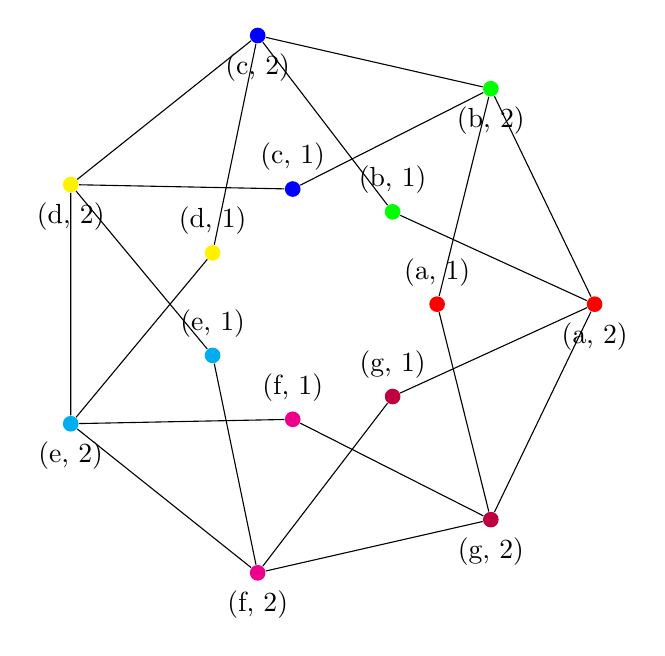
\begin{tikzpicture}
                \def\radius{1.5cm}
                \def\outerradius{3.5cm}
                \foreach \i/\color [count=\j from 0] in {(a, 1)/red, (b, 1)/green, (c, 1)/blue, (d, 1)/yellow, (e, 1)/cyan, (f, 1)/magenta, (g, 1)/purple} {
                    \node[circle, fill=\color, inner sep=2pt, label=above:\i] (v1\j) at ({360/7 * \j}:\radius) {};
                }
                \foreach \i/\color [count=\j from 0] in {(a, 2)/red, (b, 2)/green, (c, 2)/blue, (d, 2)/yellow, (e, 2)/cyan, (f, 2)/magenta, (g, 2)/purple} {
                    \node[circle, fill=\color, inner sep=2pt, label=below:\i] (v2\j) at ({360/7 * \j}:\outerradius) {};
                }
                
                \draw (v20) -- (v11);
                \draw (v21) -- (v10);
                \draw (v22) -- (v11);
                \draw (v23) -- (v12);
                \draw (v21) -- (v12);
                \draw (v22) -- (v13);
                \draw (v24) -- (v13);
                \draw (v23) -- (v14);
                \draw (v25) -- (v14);
                \draw (v24) -- (v15);
                \draw (v26) -- (v15);
                \draw (v25) -- (v16);
                \draw (v20) -- (v16);
                \draw (v26) -- (v10);
                \foreach \j in {20,...,25} {
                    \draw (v\j) -- (v\the\numexpr\j+1\relax);
                }
                \draw (v20) -- (v26);
            \end{tikzpicture}
            \caption{Example of $Z(G)$ given $G$ is $C_7$}
        \label{Fig:Main}
    \end{figure}
\end{example}
    
We can observe that routing graph $H := (Z(G), \mathcal{C}, T)$ is isomorphic to $G$ via $((x, 1) \rightarrow x)$,
and we also have copy of $G$ in induced subgraph of $Z[V(G) \times \{2\}]$. Now we study if there exists rooted $H$-certificate in 
$Z(G)$ for different graphs of $G$.

\begin{claim}
The bags of any H-certificate $c = (V_{t})_{t \in T}$ in $Z(G)$ have average order at most 2.
\end{claim}
\begin{proof}
    $|T| = |V(H)| = |V(G)|$ and $|V(Z(G))| = 2|V(G)|$, all $V_{t}$'s are pairwise disjoint, hence the average size of any bag is:
    \begin{equation}
        \frac{1}{|T|} \sum_{t \in T} |V_{t}| \leq \frac{|V(Z(G))|}{|T|} = \frac{2|V(G)|}{|V(G)|} = 2
    \end{equation}
\end{proof}

This means if we have a bag with an order 3, then there is also a bag with order 1.
And locally the inverse implications sounds almost the same.

\begin{claim}
    \label{claim:first}
    If $st \in E(H)$ is not on any triangle of $H$, then $|V_{s}| = 1 \implies |V_{t}| \geq 3$ 
\end{claim}

\begin{proof}
    Let $st \in E(H)$, and suppose $V_{s} = \{s\}$, hence $|V_{s}| = 1$, $|V_{t}| \geq 2$ because $s, t$ are not adjacent in $Z(G)$.
    If $|V_{t}| = 2$, then for $u \in V(Z(G))$, $V_{t} = \{t, u\}$, this means there is an edge $su \in E(Z(G))$ as well, at the same time 
    the corresponding $u'$ of $u$ in $V(H)$ should be adjacent with $t$, but since $s, t$ are not in a triangle of $H$, there is no edge
    between $s$ and $u'$, which means there is no $su$ edge as well, which is a contradiction. Hence $|V_{t}| \geq 3$
\end{proof}

If all the bags of the certificate have order 2, then we can look at a function $f: V(G) \to V(G)$, which for a bag $V_{(x, 1)} = \{(x, 1), (y, 2)\}$ is defined as $f(x) := y$.
Since the bags are disjoint, $f$ is an injection and therefore a permutation of $V(G)$. Since all the elements of each bag are connected we can observe
that $xf(x) \in E(G)$, and we can represent $f$ as a partial orientation of $G$, where $xy$ is oriented from $x$ to $y$ if and only if $y = f(x)$. 
For a rooted $H$-certificate $c$ in $Z(G)$ any $xy \in E(G)$ implies that $V_{(x, 1)}$ and $V_{(y, 1)}$ are adjacent, which is equivalent to say
$f(y)$ is adjacent to $f(x)$ or $x$, or $f(x)$ is adjacent to $f(y)$ or $y$. Conversely, if $f$ is a permutation of $V(G)$ with the following properties:

\begin{itemize}
    \item [\textbf{1.}] $(\forall x \in V(G)) (xf(x) \in E(G))$ 
    \item [\textbf{2.}] $xy \in G$ implies that $f(x)$ is adjacent to either $y$ or $f(y)$, or $f(y)$ is adjacent to either $x$ or $f(x)$
\end{itemize}
Then $V_{(x, 1)} = \{(x, 1), (f(x), 2)\}$ defines an $H$-vertificate in $Z(G)$.
Let's call such permutation as a `good permutation' throughout this chapter

\begin{claim}
    \label{claim:second}
    If $G$ has a good permutation, then every vertex of degree at least 3 in $G$ is on a cycle of length at most 4 in $G$
\end{claim}

\begin{proof}
    Let $f$ be good permutation and $w$ be a vertex of degree 3, let $x, y, z$ be $w$'s neighbors, WLOG $f(w) = x$ and $f(y) \neq w$.
    Let $u := f(y) \neq w$, if $u$ is adjacent to $w$, then $wyu$ form a triangle, and we are done. \newline
    Otherwise, let's assume $u$, $w$
    are not adjacent, by (\textbf{2}) condition of a `good' permutation, $f(w) = x$ is adjacent to either $y$ or $u = f(y)$, or $f(y) = u$ is adjacent
    to $f(w) = x$ or $w$, in any case $w$ will be either on $4$-cycle or $3$-cycle.
\end{proof}

\begin{thm}
    $K_{7}$ doesn't have property (*)
\end{thm}

\begin{proof}
    Let graph $G$ be a graph on 7 vertices, which is obtained by adding vertex $x$ to $C_{6}$ and adding
    2 edges to $x$ such that the endpoints of the edges are at distance 3 from each other in $C_{6}$.
    
    \begin{figure}[H]
    \centering
    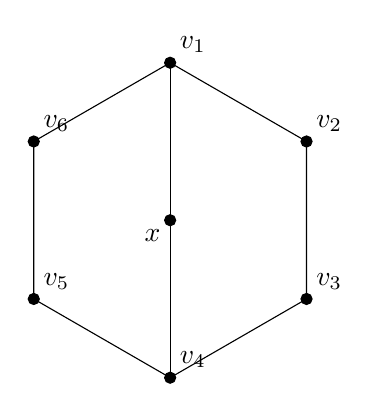
\begin{tikzpicture}[scale=1]

        \coordinate (v1) at (0,2);
        \coordinate (v2) at ({2*cos(30)},{2*sin(30)});
        \coordinate (v3) at ({2*cos(-30)},{2*sin(-30)});
        \coordinate (v4) at (0,-2);
        \coordinate (v5) at ({2*cos(-150)},{2*sin(-150)});
        \coordinate (v6) at ({2*cos(150)},{2*sin(150)});
        \coordinate (x) at (0,0);
        
        \draw (v1) -- (v2) -- (v3) -- (v4) -- (v5) -- (v6) -- cycle;
        
        \draw (x) -- (v1);
        \draw (x) -- (v4);
        
        \foreach \i in {1,...,6}{
            \filldraw (v\i) circle (2pt);
            \node[above right] at (v\i) {$v_{\i}$};
        }
        
        % Draw x
        \filldraw (x) circle (2pt);
        \node[below left] at (x) {$x$};
        
        \end{tikzpicture}
        \caption{Graph $G$ obtained from $C_6$}
    \end{figure}

    For contradiction assume that $Z(G)$ has an $H$-certificate $(V_{t})_{t \in T}$ with $T = V(G) \times \{1\}$.
    Let $A$ be the set of vertices $t \in T$ such that $|V_t| = 1$. Observe that there are 2 vertices of degree 3 in $G$,
    $v_1$ and $v_4$, and both of them are in cycle of 5, and hence by \textbf{Claim \ref{claim:second}} $G$ doesn't
    have a good permutation, which means $|A| \geq 1$. Since $|V_{t}| = 1$ for every element of $A$, it means
    $A$ is an anticlique in $H$, hence $|A| \leq 3$. By \textbf{Claim \ref{claim:first}}, $|V_s| \geq 3$ for every $s$ in $N_{H}(A)$.
    For each case of $|A| = 1$, $|A| = 2$, $|A| = 3$, it can be seen that $N_{H}(A) \geq |A| + 1$.
    \begin{itemize}
        \item $3(|A| + 1)$ is the lower bound of the number of vertices in the bags of the neighborhood of $A$, because each bag has size $\geq$ 3  and there are at least $|A| + 1$ neighbors for $A$
        \item $1|A|$ is the number of vertices of the bags of $A$, because by definition each of $A$ has size 1
        \item $2(7 - (|A| + 1) - |A|)$ is the number of vertices in the rest of the bags. Which all have $|V_t| = 2$
    \end{itemize}
    Let's denote $q$ the number of vertices in the bags of $Z(G)$ which form $H$. And let's count it.
    \begin{equation}
        q = \sum_{t \in T} |V_t| \geq 3(|A| + 1) + 2(7 - (|A| + 1) - |A|) + 1|A| = 15
    \end{equation}
    At the same time, $q \leq |V(Z(G))| = 14$, causing a contradiction. Hence, the graph $G$ doesn't have property (*),
    and since all the subgraphs of a graph with property (*) have the proprety as well, this implies that $K_7$ doesn't have 
    property (*).
\end{proof}